\documentclass[a4paper,UTF8]{article}
\usepackage{ctex}
\usepackage[margin=1.25in]{geometry}
\usepackage{color}
\usepackage{graphicx}
\usepackage{amssymb}
\usepackage{amsmath}
\usepackage{amsthm}
\usepackage{enumerate}
\usepackage{bm}
\usepackage{hyperref}
\numberwithin{equation}{section}
%\usepackage[thmmarks, amsmath, thref]{ntheorem}
\theoremstyle{definition}
\newtheorem*{solution}{Solution}
\newtheorem*{prove}{Proof}
\newcommand{\indep}{\rotatebox[origin=c]{90}{$\models$}}

\usepackage{multirow}

%--

%--
\begin{document}
\title{机器学习导论\\
习题五}
\author{141220120, 徐世坚, xsj13260906215@gmail.com}
\maketitle
\section{[25pts] Bayes Optimal Classifier}
试证明在二分类问题中,但两类数据同先验、满足高斯分布且协方差相等时,LDA可产生贝叶斯最优分类器。
\begin{solution}
此处用于写证明(中英文均可)\\
已知两类数据同先验,满足高斯分布且协方差相同,设方差均为$\Sigma$\\
贝叶斯最优分类器要求选择使后验概率$P(c|\mathbf{x})$最大的类别标记。\\
$P(c|\mathbf(x))=\frac{P(c)P(\mathbf{x}|c)}{P(\mathbf{x})}$,又$P(\mathbf{x})$对所有类别都相同,所以舍去。\\
对上述化简后的式子取对数,同时,因为先验分布相同,所以舍去$log(P(c))$项,则,对于贝叶斯最优分类器来说,第$i$类的决策函数为:\\
$f_i=\mathbf{x}^T\Sigma^{-1}\mathbf{\mu}_i - \frac{1}{2}\mathbf{\mu}_i^T \Sigma^{-1}\mathbf{\mu}_i$\\
所以,贝叶斯最优分类器的判别函数为:\\
$f=f_0-f_1=\mathbf{x}^T\Sigma^{-1}\mathbf{\mu}_0 - \frac{1}{2}\mathbf{\mu}_0^T \Sigma^{-1}\mathbf{\mu}_0  -  \mathbf{x}^T\Sigma^{-1}\mathbf{\mu}_1 + \frac{1}{2}\mathbf{\mu}_1^T \Sigma^{-1}\mathbf{\mu}_1$\\
$\qquad = \mathbf{x}^T\Sigma^{-1}(\mathbf{\mu}_0-\mathbf{\mu}_1) + \frac{1}{2}\mathbf{\mu}_1^T \Sigma^{-1}\mathbf{\mu}_1 - \frac{1}{2}\mathbf{\mu}_0^T \Sigma^{-1}\mathbf{\mu}_0$\\
下面考虑FLD。由FLD的计算可知,$\mathbf{\omega} = (\Sigma_0 + \Sigma_1)^{-1}(\mathbf{\mu}_0 - \mathbf{\mu}_1) = \frac{1}{2}\Sigma^{-1}(\mathbf{\mu}_0 - \mathbf{\mu}_1)$\\
所以,FLD的判别函数为:\\
$\mathbf{\omega}(\mathbf{x}- \frac{1}{2}(\mathbf{\mu}_0 + \mathbf{\mu}_1)$\\
$=\mathbf{x}^T\mathbf{\omega} - \frac{1}{2}(\mathbf{\mu}_0 + \mathbf{\mu}_1)^T\mathbf{\omega}$\\
$=\frac{1}{2}\mathbf{x}^T\Sigma^{-1}(\mathbf{\mu}_0 - \mathbf{\mu}_1) - \frac{1}{4} (\mathbf{\mu}_0 + \mathbf{\mu}_1) \Sigma^{-1} (\mathbf{\mu}_0 - \mathbf{\mu}_1)$\\
$=\frac{1}{2} (\mathbf{x}^T\Sigma^{-1}(\mathbf{\mu}_0-\mathbf{\mu}_1) + \frac{1}{2}\mathbf{\mu}_1^T \Sigma^{-1}\mathbf{\mu}_1 - \frac{1}{2}\mathbf{\mu}_0^T \Sigma^{-1}\mathbf{\mu}_0)$\\
得到的形式和贝叶斯最优分类器的形式是一样的,只是多了常数项$\frac{1}{2}$.\\
所以,二分类任务中两类数据满足高斯分布,且方差相同、先验相同时,线性判别分析产生贝叶斯最优分类器。\\
\end{solution}

\section{[25pts] Naive Bayes}
考虑下面的400个训练数据的数据统计情况,其中特征维度为2($\mathbf{x}=[x_1,x_2]$),每种特征取值0或1,类别标记$y\in\{-1,+1\}$。详细信息如表\ref{table:training}所示。

根据该数据统计情况,请分别利用直接查表的方式和朴素贝叶斯分类器给出$\mathbf{x}=[1,0]$的测试样本的类别预测,并写出具体的推导过程。
\begin{table}[h]
\centering
\caption{数据统计信息}
\label{table:training}\vspace{2mm}
\begin{tabular}{cc|cc}\hline
$x_1$		&  $x_2$ 	&	$y=+1$	&	$y=-1$ 	\\ \hline
0		&  0 	&	90	&	10 \\
0		&  1 	&	90 	&	10 \\
1		&  0 	&	51 	&	49 \\
1		&  1 	&	40 	&	60 \\\hline
\end{tabular}
\end{table}

\begin{solution}
此处用于写解答(中英文均可)\\
直接查表可知:\\
$P(y=+1|x=[1,0])=\frac{51}{100},P(y=-1|x=[1,0])=\frac{49}{100}$\\
$\therefore$样本$\mathbf{x}=[1,0]$的预测类别是$y=+1$.\\
$P(y=+1)=\frac{271}{400} \quad P(y=-1)=\frac{129}{400}$\\
$P(x_1=0|y=+1)=\frac{180}{271} \quad P(x_1=1|y=+1)=\frac{91}{271}$\\
$P(x_2=0|y=+1)=\frac{141}{271} \quad P(x_2=1|y=+1)=\frac{130}{271}$\\
$P(x_1=0|y=-1)=\frac{20}{129} \quad P(x_1=1|y=-1)=\frac{109}{129}$\\
$P(x_2=0|y=-1)=\frac{59}{129} \quad P(x_2=1|y=-1)=\frac{70}{129}$\\
$P(y=+1)\prod_{i=1}^{2}P(x_i|y=+1)=P(y=+1)P(x_1=1|y=+1)P(x_2=0|y=+1)=0.1184$\\
$P(y=-1)\prod_{i=1}^{2}P(x_i|y=-1)=P(y=-1)P(x_1=1|y=-1)P(x_2=0|y=-1)=0.1246$\\
$\therefore$样本$\mathbf{x}=[1,0]$的预测类别是$y=-1$
\end{solution}

\section{\textbf{[25pts]} Bayesian Network}
贝叶斯网(Bayesian Network)是一种经典的概率图模型,请学习书本7.5节内容回答下面的问题:

(1) \textbf{[5pts]} 请画出下面的联合概率分布的分解式对应的贝叶斯网结构:
\begin{equation*}
\Pr(A, B, C, D, E, F, G) = \Pr(A)\Pr(B)\Pr(C)\Pr(D|A)\Pr(E|A)\Pr(F|B, D)\Pr(G|D, E)
\end{equation*}

(2) \textbf{[5pts]} 请写出图\ref{fig-DAG}中贝叶斯网结构的联合概率分布的分解表达式。
\begin{figure}[h]
\centering
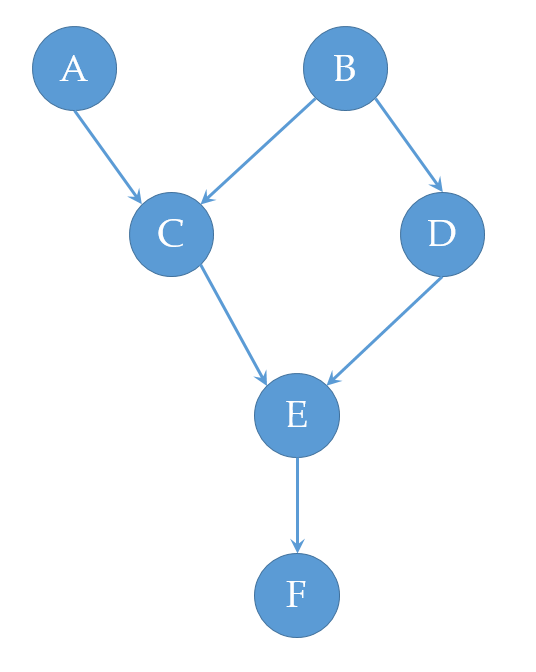
\includegraphics[scale=0.3]{bayes_net.png}
\caption{题目3-(2)有向图}
\label{fig-DAG}
\end{figure}

(3) \textbf{[15pts]} 基于第(2)问中的图\ref{fig-DAG}, 请判断表格\ref{table:DAG}中的论断是否正确,只需将下面的表格填完整即可。
\begin{table}[h]
\centering
\caption{判断表格中的论断是否正确}
\label{table:DAG}
\begin{tabular}{c|l|c||c|l|c}\hline
序号   		& 		关系  			& True/False 	& 序号   	& 		关系  			& True/False \\ \hline
1			&	$A \indep B$ 		    & 	T		    & 7  		& 	$F \perp B|C$ 		& 	F		 \\
2			&	$A \perp B|C$ 	    & 	F		    & 8  		& 	$F \perp B|C, D$ 	& 	T		 \\
3			&	$C \indep D $		    & 	F		    & 9  		& 	$F \perp B|E$ 		& 	T		 \\
4			&	$C \perp D|E$ 	    & 	F		    & 10  		& 	$A \indep F $			& 		F	 \\
5			&	$C \perp D|B, F$     & 		F	    & 11  		& 	$A \perp F|C$ 		& 	F		 \\
6			&	$F \indep B $		    & 	F		    & 12  		& 	$A \perp F|D$ 		& 	F		 \\ \hline
\end{tabular}
\end{table}

\begin{solution}
此处用于写解答(中英文均可)\\
(1)\\
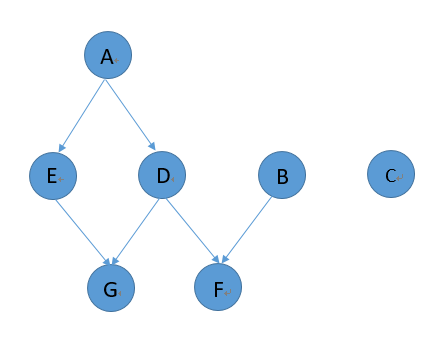
\includegraphics[height=6cm]{pic.png}\\
(2)$P_r(A,B,C,D,E,F)=P_r(A)P_r(B)P_r(C|A,B)P_r(D|B)P_r(E|C,D)P_r(F|E)$\\
(3)见填表。
\end{solution}


\section{[25pts] Naive Bayes in Practice}
请实现朴素贝叶斯分类器,同时支持离散属性和连续属性。详细编程题指南请参见链接:\url{http://lamda.nju.edu.cn/ml2017/PS5/ML5_programming.html}. 

\end{document}